\begin{figure}
        \centering
        \begin{subfigure}[b]{0.5\textwidth}
                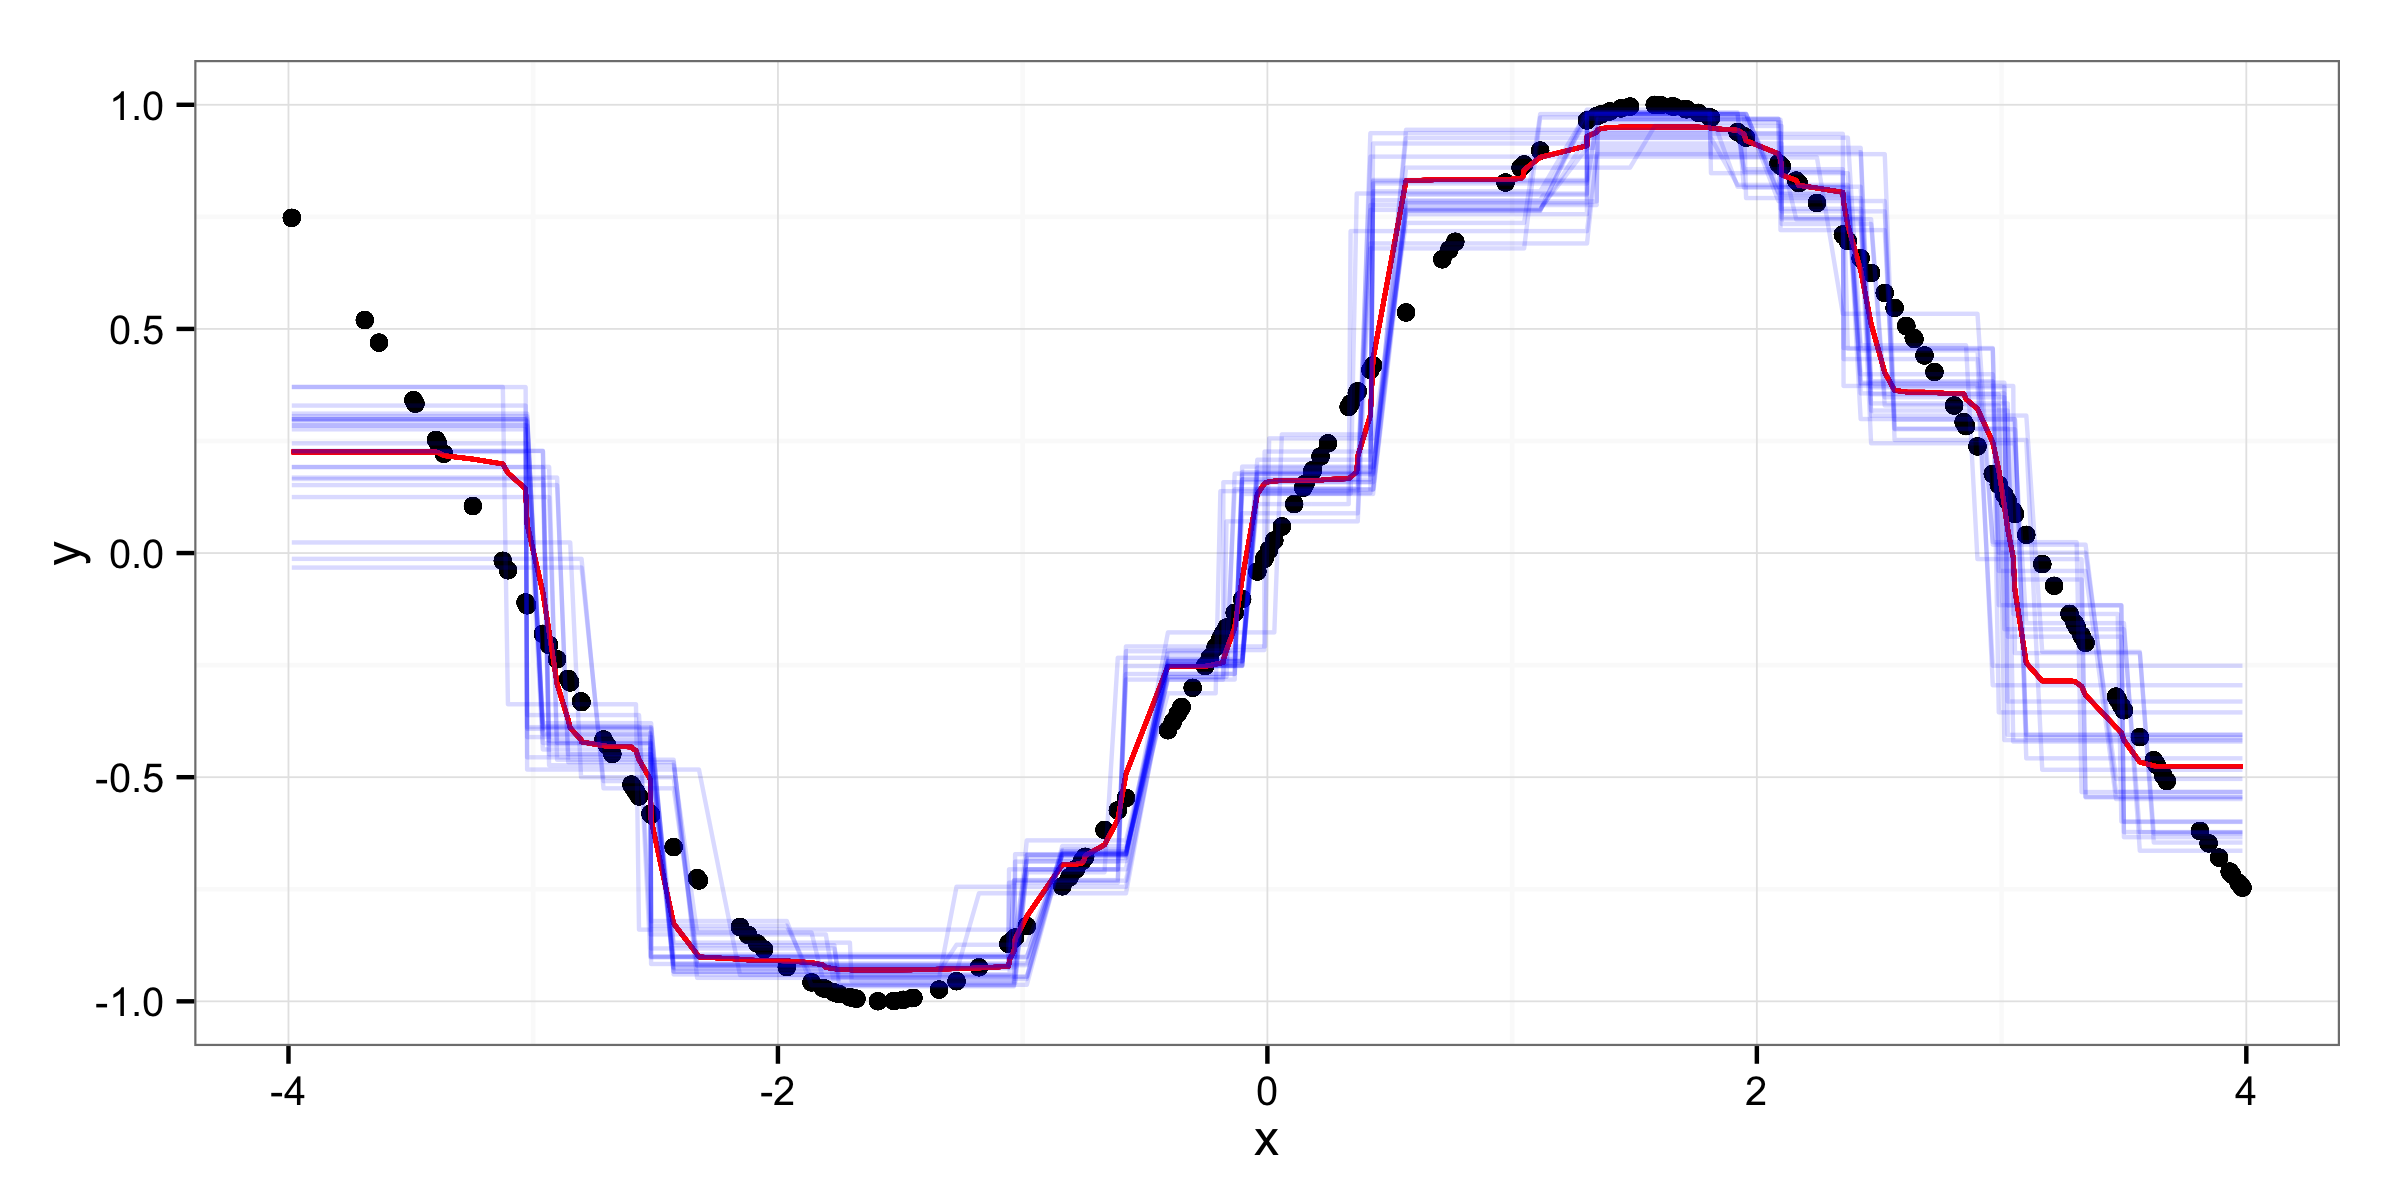
\includegraphics[width=\textwidth]{figures/forest_approximation.png}
                \caption{Approximating $\mathbf{y} = \sin(\mathbf{x}) + \epsilon$ with a regression tree which is a piecewise constant function.}
                \label{fig:cart_approx}
        \end{subfigure}%
        ~ %add desired spacing between images, e. g. ~, \quad, \qquad, \hfill etc.
          %(or a blank line to force the subfigure onto a new line)
        \begin{subfigure}[b]{0.5\textwidth}
                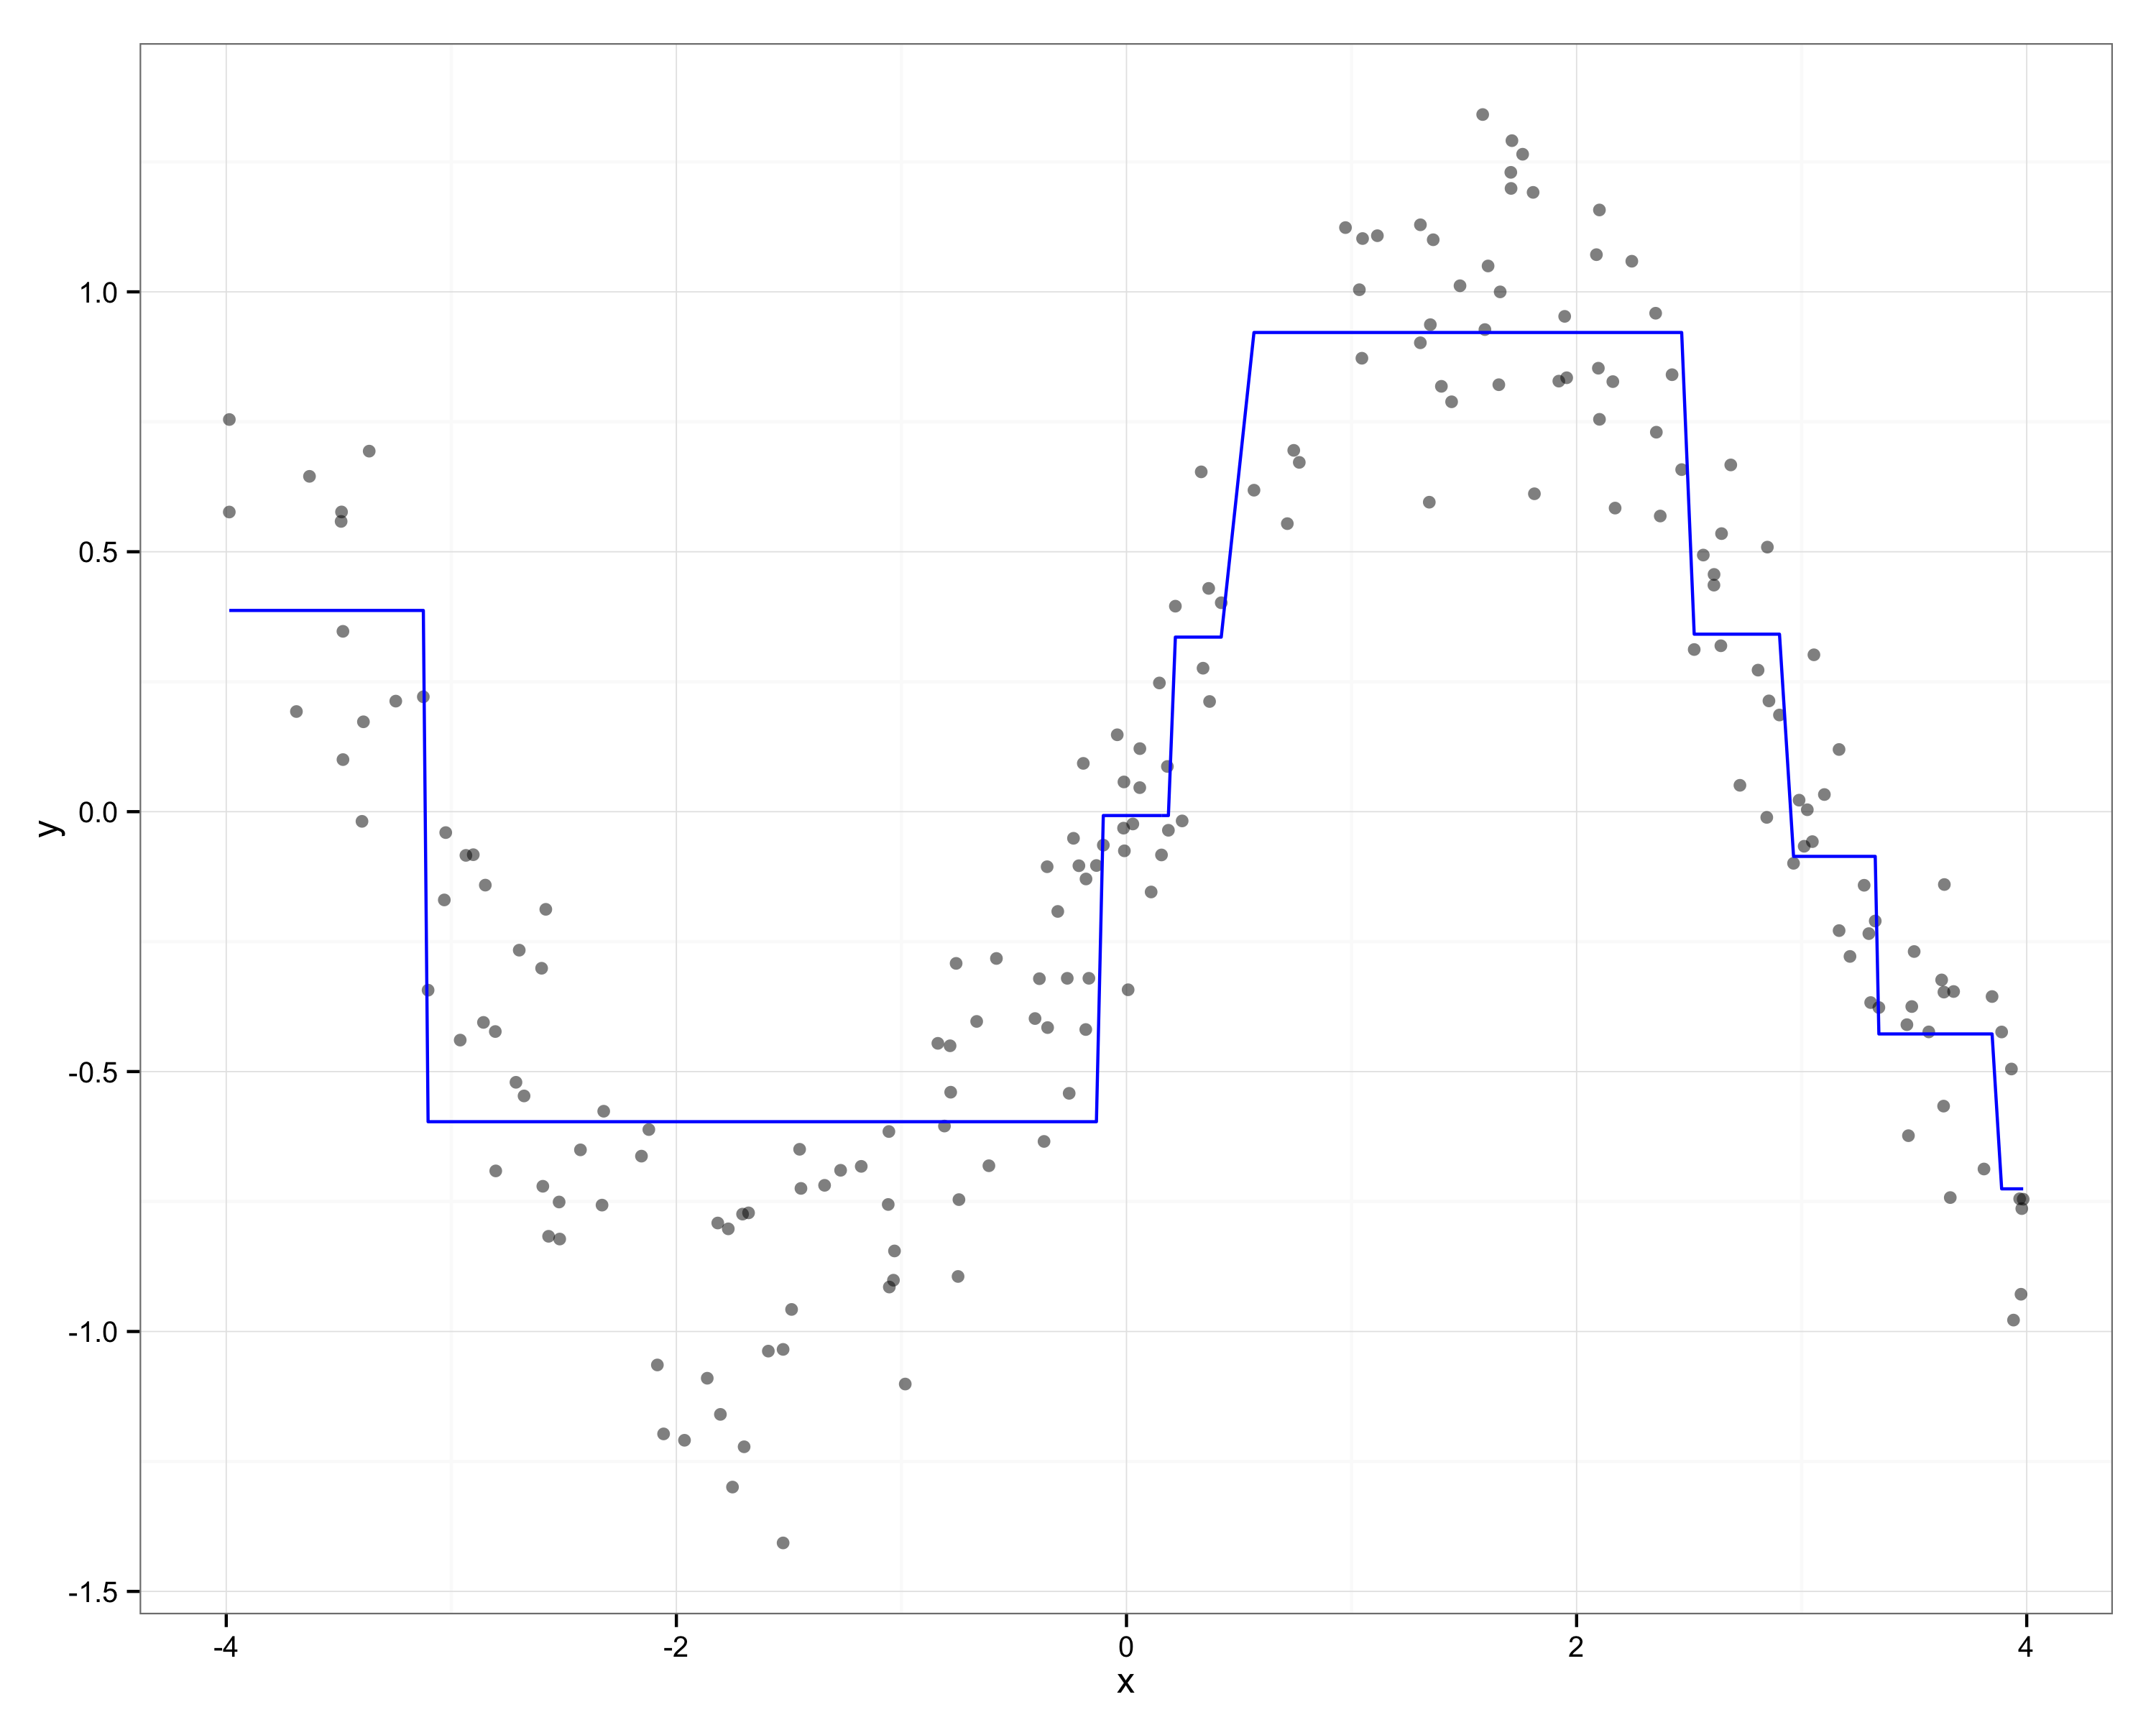
\includegraphics[width=\textwidth]{figures/cart_approximation.png}
                \caption{25 randomly selected trees (shown in blue) in a Random Forest (prediction shown in red) each grown with a subsample (.632) of the training data.}
                \label{fig:rf_approx}
        \end{subfigure}
        \caption{Demonstration of piecewise constant function approximation with CART and Random Forest.}
        \label{fig:interaction}
\end{figure}
